\documentclass[titlepage, a4paper, 12pt, reqno, openany]{report}
%\documentclass[12pt]{report}
%%%%%%%%%%%%%%%%%%%%%%%%%%%%%%%%%%%%%%%%%%%%%%%%%%%%%%%%%%%%%%%%%%%%%%%%%%%%%
\usepackage{titlepic}
%%%%%%encoding%%%%%%
\usepackage[T1]{fontenc}
\usepackage[utf8]{inputenc}
\usepackage{hyphenat}
\usepackage[portuguese]{babel}
%%%%%%Hyphenation rules%%%%%%
\usepackage{graphicx} %permite inserir figuras
\usepackage{caption}
%\usepackage{subcaption}
\usepackage{color,colortbl,multirow}
\usepackage[top=2cm,left=1cm,right=1cm,bottom=2cm]{geometry}
%\usepackage[margin=2cm]{geometry} %margens
%\usepackage[left=2cm,top=1cm,bottom=2cm,right=3cm,nohead,nofoot]{geometry}
\usepackage{paralist}
\usepackage{float}
\usepackage{verbatim}
\usepackage{lipsum}
\usepackage{multicol}
\usepackage{babelbib}
\usepackage{amsfonts}
\usepackage{amsmath}
\usepackage{amssymb}
%%%%%%%%%%%%%%%%%%%%%%%%%%%%%%%%%%%%%%%%%%%%%%%%%%%%%%%%%%%%%%%%%%%%%%%%%%%%%%%
\usepackage[usenames,dvipsnames,svgnames,table]{xcolor} %\usepackage[usenames]{color} %permite letras coloridas
%\usepackage{times}
%\usepackage{makeidx} %para criar índice remissivo
%\usepackage{array}
%\usepackage{supertabular}
%\usepackage{bm}
%\usepackage{booktabs}
%\usepackage{boxedminipage}
%\usepackage{caption}
%\usepackage{changepage}
%\usepackage{cite}
%\usepackage{easylist}
%\usepackage{esint}
%\usepackage{eucal}
%\usepackage{fancyhdr}
%\usepackage{hyperref} %index dentro de red boxes
%\usepackage{indentfirst}
%\usepackage{latexsym}
%\usepackage{listings}
%\usepackage{mathptmx}
%\usepackage{mathrsfs} %permite o uso de letras trabalhadas
%\usepackage{microtype}
%\usepackage[normalem]{ulem} %permite sublinhar palavras
%\usepackage{pifont}
%\usepackage{rotating}
%\usepackage{setspace}
%\usepackage{syntonly} %speedup work desabling pdf converse \syntaxonly
%\usepackage{subfiles}
%\usepackage{textcomp}
%\usepackage{theorem}
%\usepackage{ulem}
%\usepackage{url}
%\usepackage{wrapfig}
%%%%%recent%%%%%
%\usepackage{cancel}
%\usepackage[fleqn]{mathtools}
%\usepackage{pdfpages}
%\usepackage{pdflscape}
%\usepackage{todonotes}
%\usepackage{siunitx}
%%%%%%%%%%%%%%%%%%%%%%%%%%%%%%%%%%%%%%%%%%%%%%%%%%%%%%%%%%%%%%%%%%%%%%%%%%%%%%%%%%%
%\renewcommand\thesection{\arabic{section}}
%\renewcommand\thesubsection{\thesection.\arabic{subsection}}
%%%%%%%%%%%%%%%%%%%%%%%%%%%%%%%%%%%%%%%%%%%%%%%%%%%%%%%%%%%%%%%%%%%%%%%%%%%%%%%%%%%%
%\usepackage{enumitem}
\begin{comment}
\setlistdepth{12}
\newlist{enumitem}{enumerate}{12}
\setlist[enumitem,1]{label=\roman*)}
\setlist[enumitem,2]{label=\alph*)}
\setlist[enumitem,3]{label=\arabic*)}
\setlist[enumitem,4]{label=(\roman*)}
\setlist[enumitem,5]{label=(\alph*)}
\setlist[enumitem,6]{label=(\arabic*)}
\setlist[enumitem,7]{label=\roman*)}
\setlist[enumitem,8]{label=\alph*)}
\setlist[enumitem,9]{label=\arabic*)}
\setlist[enumitem,10]{label=(\roman*)}
\setlist[enumitem,11]{label=(\alph*)}
\setlist[enumitem,12]{label=(\arabic*)}
\end{comment}

%%%%%%%%%%%%%%%%%%%%%%%%%%%%%%%%%%%%%%%%%%%%%%%%%%%%%%%%%%%%%%%%%%%%%%%%%%%%%%%%%%%%
%\usepackage{enumerate}
\begin{comment}
\renewcommand{\labelitemi}{$\bullet$}
\renewcommand{\labelitemii}{$\cdot$}
\renewcommand{\labelitemiii}{$\diamond$}
\renewcommand{\labelitemiv}{$\ast$}
\end{comment}

%%%%%%%%%%%%%%%%%%%%%%%%%%%%%%%%%%%%%%%%%%%%%%%%%%%%%%%%%%%%%%%%%%%%%%%%%%%%%%%%%%%%
\usepackage{tikz}
\usepackage{circuitikz}
\usetikzlibrary{matrix,shapes.geometric,arrows,trees,positioning,calc}
\begin{comment}
\tikzstyle{RECTANGLE_2} = [rectangle, draw, text width=5em, text centered, rounded corners, minimum height=4em]
\tikzstyle{RECTANGLE_3} = [rectangle, rounded corners, minimum width=3cm, minimum height=1cm,text centered, draw=black, fill=red!80]
\tikzstyle{RECTANGLE_4} = [rectangle, draw, fill=blue!20, text width=3cm, text centered, minimum height=4em]
\tikzstyle{RECTANGLE_5} = [rectangle, minimum width=3cm, minimum height=1cm, text centered, text width=3cm]
\tikzstyle{RECTANGLE_6} = [rectangle, draw, fill=blue!20, text width=5em, text centered, rounded corners, minimum height=4em]
\tikzstyle{RECTANGLE_7} = [rectangle, draw, fill=blue!20, text width=5em, text centered, rounded corners, minimum height=4em]
\tikzstyle{RECTANGLE_8} = [rectangle, draw, align=left, fill=blue!20]
\tikzstyle{RECTANGLE_1} = [rectangle, rounded corners, minimum width=1cm, minimum height=1cm,text centered, draw=black, fill=green!%30]
\tikzstyle{DIAMOND_1} = [diamond, draw, fill=blue!20, text width=4.5em, text badly centered, node distance=4cm, inner sep=0pt]
\tikzstyle{DIAMOND_2} = [diamond, minimum width=3cm, minimum height=1cm, text centered, draw=black, fill=green!30]
\tikzstyle{DIAMOND_3} = [diamond, draw, text width=4.5em, text badly centered, node distance=3cm, inner sep=0pt]
\tikzstyle{DIAMOND_4} = [diamond, draw, fill=blue!20, text width=4.5em, text badly centered, node distance=3cm, inner sep=0pt]
\tikzstyle{DIAMOND_5} = [diamond, draw, fill=blue!20, text width=4.5em, text badly centered, node distance=3cm, inner sep=0pt]
\tikzstyle{DIAMOND_6} = [diamond, draw, fill=blue!20, text width=4.5em, text badly centered, node distance=4cm, inner sep=0pt]
\tikzstyle{DIAMOND_7} = [diamond, draw, align=left, fill=blue!20]
\tikzstyle{ELLIPSE_1} = [draw, ellipse,fill=red!20, node distance=3cm, minimum height=2em]
\tikzstyle{ELLIPSE_2} = [draw, ellipse,fill=red!20, node distance=3cm, minimum height=2em]
\tikzstyle{ELLIPSE} = [draw, ellipse,fill=red!20, node distance=3cm, minimum height=2em]
\tikzstyle{TRAPEZIUM_1} = [trapezium,trapezium left angle=70,trapezium right angle=-70,minimum height=0.6cm, draw, fill=blue!20, text width=4.5em, text badly centered, node distance=3cm, inner sep=0pt]
\tikzstyle{TRAPEZIUM_2} = [trapezium, trapezium left angle=70, trapezium right angle=110, minimum width=3cm, minimum height=1cm, text centered, draw=black, fill=blue!30]
\tikzstyle{TRAPEZIUM_3} = [trapezium,trapezium left angle=70,trapezium right angle=-70,minimum height=0.6cm, draw, fill=blue!20, text width=4.5em, text badly centered, node distance=3cm, inner sep=0pt]
\tikzstyle{ARROW} = [thick,->,>=stealth]
\tikzstyle{LINE} = [draw, -latex']
\tikzstyle{MYLINE} = [draw, ->,  thick, shorten <=4pt, shorten >=4pt]
\tikzstyle{TEXT_1}=[draw,text centered,minimum size=6em,text width=5.25cm,text height=0.34cm]
\tikzstyle{TEXT_2}=[draw,text centered,minimum size=2em,text width=2.75cm,text height=0.34cm]
\tikzstyle{TEXT_3}=[draw,minimum size=2.5em,text centered,text width=3.5cm]
\tikzstyle{TEXT_4}=[draw,minimum size=3em,text centered,text width=6.cm]
\tikzstyle{CIRCLE_1}=[draw,shape=circle,inner sep=2pt,text centered, node distance=3.5cm]
\tikzstyle{CIRCLE_2}=[draw,shape=circle,inner sep=4pt,text centered, node distance=3.cm]
\end{comment}

%%%%%%%%%%%%%%%%%%%%%%%%%%%%%%%%%Not Adviced%%%%%%%%%%%%%%%%%%%%%%%%%%%%%%%%%%%%%%%%
%\usepackage{showidx} %for troubleshooting index
%\usepackage{showkeys} %for troubleshooting \label \ref
%\usepackage{pxfonts}

%%%%%%%%%%%%%%%%%%%%%%%%%%%%%%%%%claching Package%%%%%%%%%%%%%%%%%%%%%%%%%%%%%%%%%%%
%\usepackage{pgfplots}
%\usepackage{natbib}
%\usepackage[usenames]{color} %permite letras coloridas
%\usepackage{xypic}

%%%%%%%%%%%%%%%%%%%%%%%%%%%%%%%%%Not Installed Yet%%%%%%%%%%%%%%%%%%%%%%%%%%%%%%%%%%

%%%%%%%%%%%%%%%%%%%%%%%%%%%%%%%Com Dependencias%%%%%%%%%%%%%%%%%%%%%%%%%%%%%%%%%%%%%
%\usepackage{glossaries}
%\usepackage[version=3]{mhchem}

%%%%%%%%%%%%%%%%%%%%%%%%%%%%%%%%%%%%%%%%%%%%%%%%%%%%%%%%%%%%%%%%%%%%%%%%%%%%%%%%%%%%
% alguns pacotes nao sao reconhecidos, ter atencao quais usar em differents computadores, tambem alguns pacotes entram em conflito.
\newtheorem{theorem}{Theorem}
\newtheorem{lemma}{Lemma}
\newtheorem{definition}{Defini\c{c}\~{a}o}
\newtheorem{notation}{Notation}

%%%%%%%%%%%%%%%%%%%%%%%%%%%%%%%%Not Working%%%%%%%%%%%%%%%%%%%%%%%%%%%%%%%%%%%%%%%%%
%\usepackage{itemize}
%\usepackage{named}
%\usepackage{amscls}
%\usepackage{fullpage}

%%%%%%%%%%%%%%%%%%%%%%%%%%%%%%%%%%%%%%%%%%%%%%%%%%%%%%%%%%%%%%%%%%%%%%%%%%%%%%%%%%%%
%\usepackage{apacite} %Bibliography style
%%%%%%%%%%%%%%%%%%%%%%%%%%%%%%%%%%%%%%%%%%%%%%%%%%%%%%%%%%%%%%%%%%%%%%%%%%%%%%%%%%%%
\makeindex
%%%%%%%%%%%%%%%%%%%%%%%%%%%%%%%%%%%%%%%%%%%%%%%%%%%%%%%%%%%%%%%%%%%%%%%%%%%%%%%%%%%%
\begin{document}
%\bibliographystyle{apacite}
\bibliographystyle{babplain}
%%%%%%%%%%%%%%%%%%%%%%%%%%%%%%%FIX SECTION NUMBERING%%%%%%%%%%%%%%%%%%%%%%%%%%%%%%%%
\renewcommand\thesection{\arabic{section}}
\renewcommand\thesubsection{\thesection.\arabic{subsection}}
\renewcommand\thesubsubsection{\thesection.\thesubsection.\arabic{subsubsection}}

\begin{minipage}{\linewidth}

\title{Comportamento Organizacional}
\author{
\emph{S\'{e}rgio Santos},\;$N^o$:\; 1020881 \\
\emph{Nome 2},\;$N^o$:\; 2000000\\
\emph{Nome 3},\;$N^o$:\; 3000000\\
%\emph{Nome 4},\;$N^o$:\; 4000000\\
%\emph{Nome 5},\;$N^o$:\; 5000000\\
}
\date{\today}
%\titlepic{
\includegraphics[scale=0.50]{./image/ROQ/ROQ.jpg}}

\begin{titlepage}

\includegraphics[scale=0.60]{./image/capa/ISEP_marca_cor_grande.png}
\maketitle
\vspace{8cm}
\begin{flushleft}

\includegraphics[scale=0.50]{./image/ROQ/ROQ.jpg}
\end{flushleft}
\end{titlepage}

\end{minipage}

\tableofcontents
%\appendix
\pagestyle{plain} %plain headings empty
%\setcounter{chapter}{0}
%\numberwithin{page}{section}
%\renewcommand{\abstractname}{Executive Summary}
\setlength{\parindent}{0in}
%%%%%%%%%%%%%%%%%%%%%%%%%%%%%%%%%%%%%%%%%%%%%%%%%%%%%%%%%%%%%%%%%%%%%%%%%%%%%%%%%%%%%%%%%%%%%%%%%%%
\newpage
\label{Resumo}
\begin{abstract}
Este trabalho consiste na análise de uma organização, quanto ao Comportamento e Cultura Organizacional.\\

A Cultura Organizacional é fundamental para as organizações poder evoluir e atingir seus objetivos com sucesso. O estudo das culturas presentes nas organizações e formas de à moldar para melhor servir a sociedade e mercado sera abordado neste relatório.
\end{abstract}


%%%%%%%%%%%%%%%%%%%%%%%%%%%%%%%%%%%%%%%%%%%%%%%%%%%%%%%%%%%%%%%%%%%%%%%%%%%%%%%%%%%%%%%%%%%%%%%%%%%
\newpage
\section{Introdução}
A Empresa que vai ser abordada é a {\textcolor{blue} ROQ}\\
\\
Localizada no coração do Vale do Ave, a S. Roque - Máquinas e Tecnologia Laser S.A., labora em instalações próprias com uma área coberta de aproximadamente 25.000 m2. A empresa orgulha-se de ser hoje uma experiente e bem-sucedida PME, tendo sido distinguida pelo IAPMEI como PME Líder e de Excelência pelo quarto ano consecutivo.\\\
\\
Líder nacional no seu campo de atividade – fabrico de máquinas e equipamentos para as indústrias de estamparia têxtil e embalagem - emprega atualmente mais de 350 funcionários distribuídos pelos seus diferentes departamentos.\\
\\
Com instalações funcionais e com profissionais qualificados e experientes, a S.Roque dispõe das mais avançadas ferramentas e tecnologias na área da metalomecânica, do design e da elaboração de produto. Os equipamentos fabricados são de conceção própria, desenhados por um departamento técnico altamente especializado para corresponder aos desígnios de projeto e com o objetivo de satisfazer qualitativamente as solicitações do cliente mais exigente.\\
\\
Hoje, após a conquista e solidificação incontestável da liderança do mercado português, tornando-se num dos líderes mundiais na área da estamparia e da embalagem, a S. Roque produz e comercializa um extenso catálogo com diferentes produtos e trabalha com clientes/ parceiros um pouco em todo o mundo: Espanha, França, Itália, Inglaterra, Alemanha, Holanda, Suécia, Romênia, África do Sul, Marrocos, Tunísia, Angola, Turquia, Kuwait, Índia, China, Vietnam, Malásia, Camboja, Rússia, Bulgária, Brasil, Argentina, Peru, Colômbia, Honduras, El Salvador e E.U.A.\\
\\
\begin{figure}[ht]
\begin{center}
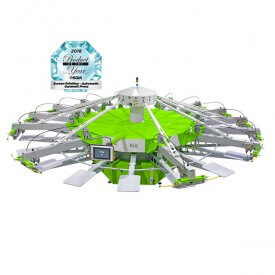
\includegraphics[scale=0.5]{"./image/ROQ/maquinas/ECO-P18_600x600-2-275x275.jpg"}
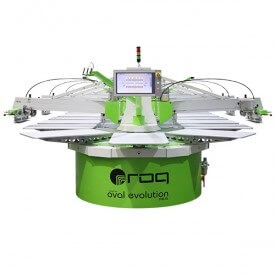
\includegraphics[scale=0.5]{"./image/ROQ/maquinas/EVO-600x600-275x275.jpg"}
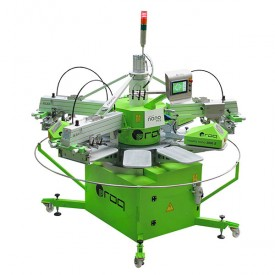
\includegraphics[scale=0.5]{"./image/ROQ/maquinas/nanop10-275x275.jpg"}
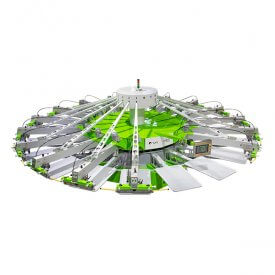
\includegraphics[scale=0.5]{"./image/ROQ/maquinas/NEXTP18-600x6001-275x275.jpg"}
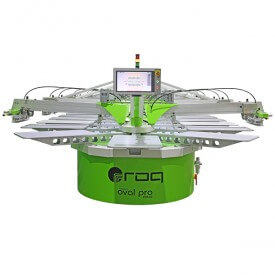
\includegraphics[scale=0.5]{"./image/ROQ/maquinas/PRO-600x600-275x275.jpg"}
\includegraphics[scale=0.5]{"./image/ROQ/maquinas/You-600x600-275x275"}
\end{center}
\end{figure}
\\
\newpage
A S. Roque dedica-se à construção e comercialização de máquinas de estamparia têxtil há mais de 30 anos. Embora a sua génese esteja ligada à manutenção destes equipamentos, rapidamente foi identificada a oportunidade de construir de raiz este tipo de máquina. Os têxteis estavam em alta no Vale do Ave, e a S.Roque aproveitou para criar um produto de qualidade para uma clientela extremamente exigente. A empresa não se contentou em servir apenas o seu nicho de mercado, desde muito cedo que procurou a internacionalização. Numa primeira fase e por motivos geográficos criou parecerias europeias, numa segunda fase e por questões culturais dedicou-se ao Brasil e América do Sul. Neste milénio tornou-se numa marca global de referência na área onde atua. Todo e qualquer mercado está ao nosso alcance.\\
Hoje mais do que nunca não chega ter o melhor produto do mercado, é também necessário apresentar um serviço excelente e acessível em qualquer ponto do globo. A S.Roque orgulha-se de procurar a excelência em tudo em que se envolve com especial destaque para a procura de soluções.\\
\\
Em 2015 a marca Sroque transformou-se em ROQ. Atendendo às necessidades do seculo XXI reconhecemos a necessidade de criar uma marca verdadeiramente global que consiga de uma forma eficaz transmitir mais de 30 anos de história, inovação, internacionalização e conhecimento.

%%%%%%%%%%%%%%%%%%%%%%%%%%%%%%%%%%%%%%%%%%%%%%%%%%%%%%%%%%%%%%%%%%%%%%%%%%%%%%%%%%%%%%%%%%%%%%%%%%%
\begin{comment}
	Durante muito tempo tem havido estudos para descobrir a formula mágica que leva as organizações ter sucesso, existe muitas abordagens com diferentes perspectivas, algumas convergem e outras divergem, e assim foram criados novos conceitos de forma a encapsular estilos e tipos de forma a poder se identicar quais são os mais propícios a ter uma maior elevada taxa de sucesso, conceitos tais como comportamento organizacional, cultura organizacional, performance organizacional, etc.\\

Tem se aplicado o método cientifico para se poder medir e quantificar suas influências, assim obtemos incertezas quantificáveis dando uma ideia qual as mais prováveis levantado novas questões e duvidas das suas interações e até possíveis novas variáveis.\\

Temos ao nosso dispor um extenso leque de trabalhos nesta matéria, até considerado exagerado, que pelo menos nos indica um caminho que vale apena percorrer e explorar, graças aos indivíduos que se dedicaram a esta disciplina.\\
\end{comment}

\newpage
\section{Organização}

1. Organização privadas com fins lucrativos\\
\\
2. Atividades de Suporte\\
As atividades de suporte são as que apoiam um bom desempenho na realização das atividades principais.\\
- atividade administrativa e financeira\\
- atividade da gestão do pessoal\\
- atividade jurídica\\
- planeamento, controlo e gestão\\
- gestão de sistemas e tecnologia\\
A atividade de suporte não contribuem diretamente para a criação do valor.\\
3. Atividades principais\\
Cadeia de valor da organização é a sequencia de atividades e fluxos de informação que uma organização e os seus fornecedores devem desenvolver para desenhar, produzir, oferecer, entregar e suportar os seus produtos, estas são as atividades principais.\\
\\
A atividade principais de qualquer empresa é que diretamente cria valor.\\
- Desenvolvimento de produtos\\
- Produção dos produtos
- assistência\\
- montagem dos produtos\\
- outsourcing\\
- transporte\\
- marketing\\
- vendas\\
\\
4. Implementação por produto\\
\\
A divisão do trabalho, permitiu a redução do tempo de aprendizagem, isto é, cada um tem as suas funções, aumentando a produtividade. Cada um executa uma parte das tarefas necessárias a fabricação.\\
\\
\\
5. tipos de hierarquias\\
matricial [produto e região]\\
\\
6. tipos de departamentalizações\\
produto e localidade\\


\begin{comment}
Uma organização é um grupo estruturado de pessoas, um grupo onde cada pessoa é responsável por tarefas bem definidas e onde existe um sistema de articulação entre elas, que desenvolve um conjunto de atividades visando a definição e prossecução de objetivos comuns (de forma continuada no tempo).\\

O objetivo das organizações é para criar valor para os seus clientes/utentes, para os detentores do seu capital, para os seus colaboradores, para os seus fornecedores e para a sociedade em geral.\\

As empresas privadas são obrigadas a oferecer valor aos seus (potenciais) clientes, aos detentores do seu capital, aos trabalhadores e aos fornecedores.\\
Nas empresas privadas, existe um forte estimulo do mercado (e da concorrência) para que ela estabeleça objetivos bem definidos e socialmente apetecidos para poder sobreviver e prosperar.\\

Nas empresas publicas, o estimulo é sentido em menor grau ou não existente, consoante o tipo e características concretas da organização.\\

Nas organizações sem fim lucrativos e/ou dependentes do estado, existe outro tipo de estimulo os interesses dos governantes, quando o estado é parceiro ou responsável pela organização, os interesses de grupos de pressão da sociedade, etc.\\

Nas organizações sem fins lucrativos os objetivos estão em permanente discusão e/ou a ser alterados, resultando uma maior indefinição sobre as atividades a desenvolver por responsáveis e por colaboradores.\\

Teoria de Geer Hofteed.\\

Best practices can come from national, say the American National Standards Institute (ANSI) or the Canadian Standards Association (CSA), or international, say ISO or Institute of Electrical and Electronics Engineers (IEEE), standards organizations, professional associa-tions, or consulting firms.\\

Eliminar desperdicio e resolução de problemas.\\

Confiança na liderança e operadores.\\

Both organizational culture and a leader’s behaviors have been identified as critical determinants of an organization’s effectiveness\\

Leaders have long been viewed as a primary influence on the creation of organizational culture (e.g. Bennis and Nanus, 1985; Schein, 1983). According to Schein (1985), the “only thing of real importance that leaders do is to create and manage culture”\\

No organization today exists in a stable environment. Current scholars, especially the
proponents of complexity theories, consider that all organizations are under the influence
of multiple changes (Brown and Eisenhardt, 1997; Burnes, 2004a; Stacey et al., 2002;
Styhre, 2002; Tetenbaum, 1998). According to these scholars, change is inherent in
human action and therefore necessarily occurs in any context of human social interactions
(Ford and Ford, 1995). As organizations are sites of continuously evolving human action,
they are in a continuous state of change and, in order to survive, must develop the ability
to continuously change themselves (Burnes, 2004b; Tsoukas and Chia, 2002).\\

Constante mudança de adaptaçao ao meio ambiente.\\

Organizational culture determines how individuals behave, what people pay attention to,
how they respond to different situations, and how they socialize with new members and
exclude those who do not fit in (Spataro, 2005) \\

acknowledge that even in US and European companies, success rates are
not spectacular regarding efforts to change vision, values, and culture or business systems
and processes (Beer and Nohria, 2000; Beer et al., 1990; Carr et al., 1996).\\

Characteristica de bons Objectivos\\
- Claros\\
- Concisos\\
- Calendarizados\\
- Atingiveis\\

Tipos de organizações\
- Organização privadas com fins lucrativos\\
- Organização privadas sem fins lucrativos\\
- Organização publicas com fins lucrativos\\
- Organização publicas sem fins lucrativos\\

tipos de hierarquias\\
tipos de departamentalizações\\
organização por processo\\

A divisão do trabalho, permitiu a redução do tempo de aprendizagem, isto é, cada um tem as suas funções, aumentando a produtividade. Cada um executa uma parte das tarefas necessarias a fabricação.\\

Gestão:\\ \\
\begin{minipage}{20cm}
\begin{minipage}{5cm}
Instrumentos
\begin{enumerate}
\item Planear
\item Organizar
\item Controlar\\ \\
\end{enumerate}
\end{minipage}
\begin{minipage}{5cm}
Funções
\begin{enumerate}
\item Liderança
\item Comuniacção
\item motivação
\item Tomada de decisão
\end{enumerate}
\end{minipage}
\end{minipage}

Cadeia de valor\\
-Actividades principais\\
-Actividades de supporte\\

Cadeia de valor da organização é a sequencia de actividades e fluxos de informação que uma organização e os seus fornecedores devem desenvolver para desenhar, produzir, oferecer, entregar e suportar os seus produtos, estas são as actividades principais.\\

As actividades de suporte são as que apoiam um bom desempenho na realização das actividades principais.\\
- actividade administrativa e financeira\\
- actividade da gestão do pessoal\\
- actividade juridica\\
- planeamento, controlo e gestão\\
- gestão de sistemas e tecnologia\\

A actividade de suporte não contribuem directamente para a criação do valor.\\

Actividades de suporte e principal.\\
funções da Gestão sã Instrumental, Comportamental e Estrutural.\\

Cumprir os objectivos é ser eficaz.\\

Para gerir a produção (planear, organizar, dirigir e controlar), há que recolher um elevado volume de informação de controlo, sendo frequentemente necessário refazer o planeamento.\\

- Implementação por projecto\\
- Implementação por processo\\
- Implementação por células\\
- Implementação por cadeia ou em linha\\
- Implementação por produto\\

Na implementação por célula de fabrico procura agrupar os produtos segundo a semelhança das suas rotinas operatórias.\\
Na implementação por processo, é possivel cada serie (ou lote) ser processado integralmente num dado centro, antes de avançar para o centro onde irá sofrer a operação de transformação seguinte.\\
A análise ABC pode ser utilizada para averiguar quais as principais encomendas responsáveis pela sobrecarga de um dado centro de trabalho.\\

Organizar é estipular quem faz o quê, atribui-se os recursos necessários para o fazer, criar um sistema de informação para verificar execução.\\
\end{comment}

\newpage
\section{Cultura Organizacional}

Os fundadores da organização tem um grande impacto no processo de formação da cultura organizacional através da imposição das suas crenças e supposições no grupo. A adopção das crenças, valores e supposições que formam a cultura da organização é depois reforçada pelos varios comportmanentos primarios dos lideres.

\subsection{Missão}
\begin{comment}
A missão de uma organização consiste na sua razão de existir, actual e futura.\\
\end{comment}
A S. Roque tem como missão a constante inovação e criação de produtos de excelência na área da estamparia têxtil à peça. Para tal, aposta em múltiplos vetores complementares: tecnologia, qualidade e recursos humanos especializados. Estimula de forma persistente a sua veia empreendedora e internacional, promovendo para isso o contínuo aperfeiçoamento do seu serviço, em qualquer parte do mundo, mantendo-se fiel aos princípios éticos e de sustentabilidade.\\

\subsection{Visão}
Trilhar um percurso sustentável de inovação, de expansão internacional, de excelência em todas as soluções que lançamos para o mercado, de qualidade absoluta, para nos mantermos como líder na nossa área de negócio.\\

\subsection{Valores}
\begin{itemize}
\item Acção dentro dos princípios morais e éticos da empresa para com os seus stakeholders.
\item Actuação sempre no interesse dos nossos parceiros de forma a promover a sua satisfação e fidelização.
\item Excelência conseguida através de trabalho de equipa, competência e responsabilidade.
\item Qualidade absoluta.
\item Inovação promovida pelo ADN empreendedor da S. Roque.
\item Sustentabilidade ambiental e segurança.
\end{itemize}



\begin{comment}
O que lhes chama a atenção e medem; suas reações a incidents criticos, allocação de meios, papeis assumidos, e partilha de informação; recompensas e delegaçao de poder; recrutamento, selecção e promoção. As lideraças chave tem como responsabilidade de modificar a cultura de forma a estar actualizada com as mudanças exigidas.\\

Aqui destingue-se dois tipos de lideres os transacionais e os de transfromação. “culture affects leadership as much as leadership affects culture”

Planear é estabelecer os objectivos a atingir e o percurso de acções.\\

A formulação, avaliação e selecção de estratégias e o desenvolvimento dos planos mais detalhados para as pôr em práctica são feitos após a definição da missão e da análise do meio ambiente da organização.\\

Ferramentas para avaliar o cumprimento dos objectivos\\
- benchmarking\\
- scorecard management\\
- Banco de Portugal\\

Metodo de demonstar o desempenho de uma organizações atraves da eficacia, eficiencia e seu rendimento.\\

Eficacia avalia em que medida os objectivos estão alinhados com a necessidades sociais que ela se propõe a satisfazer, ou seja, em que medida os seus objectivos são a tal adequados.\\

Eficiencia avalia a economia de recursos utilizados para realizar os seus objectivos, requer uma boa estruturação dos processos seguidos nas actividades, o que leva tempo e custa dinheiro.\\

Missão - SWOT Meio Ambiente (transacional e contextual(PEST)) - Objectivos - Implementação.\\

O sucesso das empresas está correlacionada positivamente com o seu planeamento.\\

Na análise do meio ambiente transacional, análisa-se o comportamento previsional das entidades com quem a organização interage.\\

Controlo.\\
O controlo pode ser encarado como um processo de aprendizagem.\\
O controlo deve servir, acima de tudo, para ajudar a garantir que os objectivos estabelecidos são atingidos.\\
Se a informação recolhida e os resultados apurados no processo de controlo não conduzem a acções de correcção quando necessário, este será não só inútil, mas até prejudicial.\\
O recurso aos sistemas de informação permite, em geral, simplificar os procedimentos de controlo.\\

Controlar é os procedimentos de verificar sua execução, estar atento a imprevistos e pronto a corecções recorrendo a re-organização e/ou novo planeamento, também pode-se optar por não fazer nada.\\
\end{comment}


\newpage
\section{Estudo da Cultura Organizacional segundo o Modelo Ogbonna \& Harris}

A cultura organizacional e os comportamentos da liderança foram identificados como pontos criticos que determinam se uma organização é eficaz.\\
\begin{comment}
No entanto a comparação entre os comportamentos dos lideres e as cultura organizacional, no impacto que tem na variável organização e a eficacia da liderança ainda não foram empiricamente examinados.\end{comment}
\\
O Modelo Ogbonna \& Harris estuda a relação entre as variáveis Estilos de liderança, Cultura organizacional e Performance organizacional. Este modelo foi derivado de um estudo empírico na Inglatera através de os procedimentos científicos e estatísticos na analise dos dados obtidos por questionários as empresas envolvidas.\\
\\
{\bf As variáveis estão abaixo descritas na qual foram consideradas no estudo.}\\
\\

\begin{minipage}[t]{.3\linewidth}
\quad Estilos de Liderança:
\begin{itemize}
\item Participativo
\item Orientado as pessoas
\item Orientado as tarefas
\end{itemize}
\end{minipage}
\begin{minipage}[t]{.3\linewidth}
\quad Tipos de Cultura:
\begin{itemize}
\item Inovadora
\item Competitiva
\item Burocrática
\item Comunitária
\end{itemize}
\end{minipage}
\begin{minipage}[t]{.3\linewidth}
\quad Medição do Sucesso:
\begin{itemize}
\item Satisfação dos Clientes
\item Taxa crescimento vendas
\item Cotação no mercado
\item Vantagens Competitivas
\item Volume de vendas
\end{itemize}
\end{minipage}
\vspace{2cm}\\


Os resultados obtidos na determinação do Estilos de liderança e tipo de Cultura Organizacional das empresas Estudadas e depois o Modelo que foi criado são mostrados nas paginas seguintes.\\



\begin{comment}
Estilos de liderança:
\begin{itemize}
\item participative leadership\\
Is gauged by the extent to which leaders allow subordinates to influence decisions by requesting input and contribution.
\item supportive leadership\\
Focuses on the degree to which the behaviour of a leader can be viewed as sympathetic, amicable, and considerate of subordinate needs
\item Instrumetal leadership\\
This measure of leadership style is akin to directive or transactional leadership and is designed to measure the extent to which leaders specify expectations, establish procedures, and allocate tasks.
\end{itemize}
\end{comment}

\newpage
\begin{figure}[H]
\centering
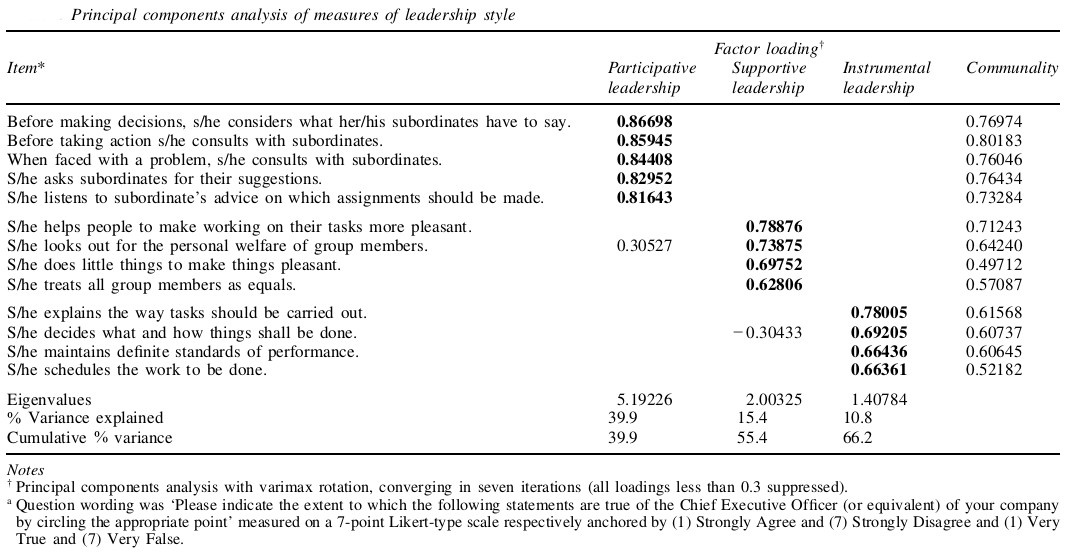
\includegraphics[scale=.5]{"./image/OB/Leadership.jpg"}\\
\caption{Estilos de Liderança, Resultado}
\label{grafico 1}
\end{figure}\par

\begin{figure}[H]
\centering
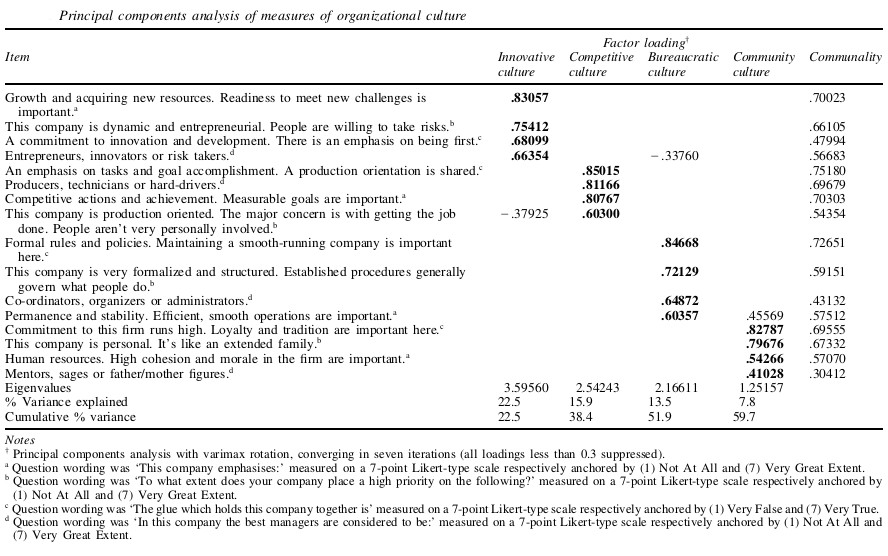
\includegraphics[scale=.6]{"./image/OB/Culture.jpg"}\\
\caption{Cultura Organizacional, Resultado}
\label{grafico 1}
\end{figure}\par

\newpage
\begin{figure}[H]
\centering
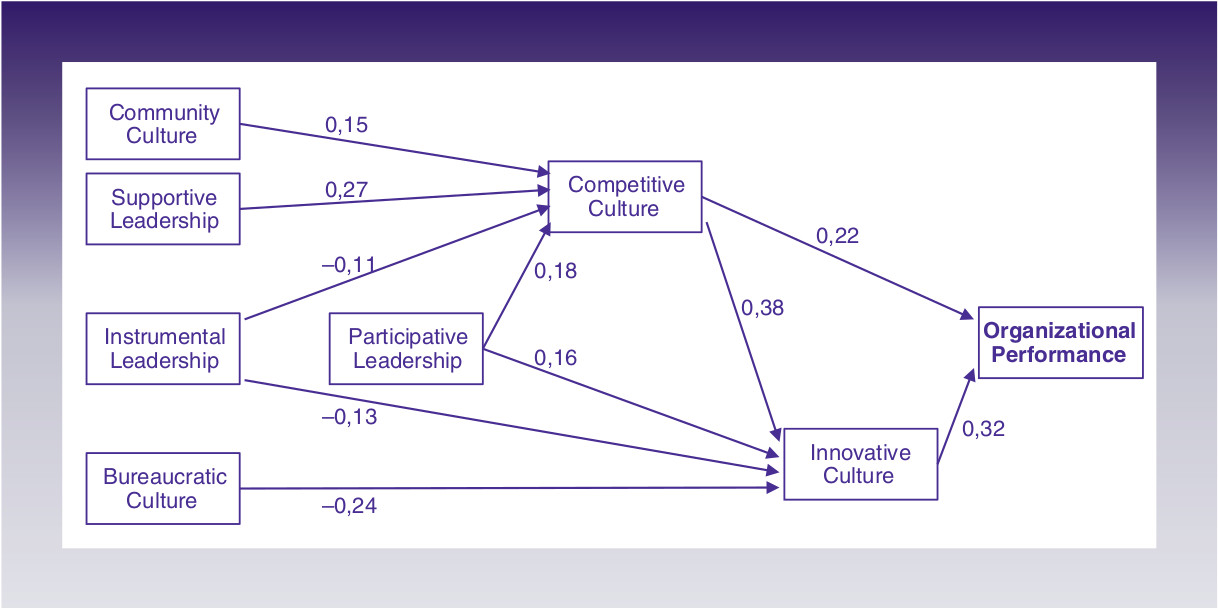
\includegraphics[scale=.4]{"./image/OB/Ogbonna & Harris.jpg"}\\
\caption{Ogbonna \& Harris, Resultado}
\label{grafico 1}
\end{figure}\par
Obtido estes dados podemos analisar a nossa organização em contraste com os resultados obtidos neste estudo.\\


\begin{comment}
Motivação teorias Moslow, Hersberg, Victor Vroom.\\
Se as condições e recompensas oferecidas aos funcionários não lhes permitirem satisfazerem algumas das suas necessidades, mais facilmente abandonam a equipa ou organizaçãoa que pertencem.\\
Motivação é o conjunto de factores que provocam, canalizam e sustentam o comportamento das pessoas.\\
Um gestor interessado em atingir um bom desempenho estabelece objectivos atingiveis e bem defenidos.\\
Auto-confiança no desenvolvimento do trabalho pode diminuir a sua motivação.\\
Motivar é criar condições necessarias para que as pessoas se empenham na prosecução dos objectivos da organização.\\
O impacto da comunicação no desempenho da organização é muito elevado.\\
Os Gestores tem de ser coerentes e alinhados com o que transmittem de forma a criar uma estrutura de confiança.\\
Um lider de uma organização é aquele que detém capacidades de influenciar os colaboradores.\\
gestão das actividades é o exercicio do poder de um gestor.\\
poder de premiar e punir é suficiente para gerir as actividades do dia a dia.\\
poder informacional.\\
Um sistema de avaliação do desempenho de uma empresa é uma valia porque é uma boa oportunidade para analisar o grau de cumprimento dos objectivos acordados.\\
A medida que as organizações se achatam, os gestores têm de aprender a permitir que os seus colaboradores tomem decisões e tenham informação sobre questões mais sensiveis.\\
Para um engenheiro é muito útil conhecr os aspectos essenciais da legislação laboral.\\
A gestão das pessoas é cada vez mais importante porque são as pessoas que têm o conhecimento e só as pessoas o podem partilhar e aplicar.\\
Numa organização, apoiar e compensar as pessoas é fundamental, mas também é indespensávelfalar com elas sobre os erros que cometem no sentido de serem corrigidas e evitadas no futuro.\\
Uma organização tem maior probabilidade de ter sucesso se gerir as pessoas de modo a que estas ao contribuirem para o sucesso da organização tenham também sucesso elas próprias.\\
A qualidade é a totalidade das caracteristicas de um produto ou serviço, que determinam a sua aptidão para satisfazer determinadas necessidades.\\
Garantia da qualidade tem como objectivo primeiro, o controlo do processo, ou seja, a minimização ou mesmo eliminação dos erros na produção.\\
A garatia da qualidade concentra-se no controlo do processo produtivo e controlo do produto.\\
Os custos relacionados com a insatisfação dos clientes são considerados custos de não qualidade.\\
O diagrama de Pareto permite identificar rapidamente as causas vitais e as triviais de um dado problema.\\
As cartas de controlo destinam-se a detectar as variações resultantes da alteração, frequentemente de natureza aleatória e acidental, de algum dos parametros de processo de fabrico (ditas causas especiais).\\
As sete ferramentas classicas da qualidade\\
- Fluxograma\\
- Registo e análise de dados\\
- Diagrama de causa - efeito (espinha de peixe 4M)\\
- Diagrama de Pareto\\
- Histogramas\\
- Diagramas de dispersão\\
- Cartas de Controlo\\
tipos de lideres\\
- Autocratico\\
- Paricipativo \\
- Democratico \\
- Deixa andar\\
estilo de lider\\
- Orientado as pessoas\\
- Orientado as tarefas\\
In their well-known and prestigious study on the relationship between leadership style , organizational culture and performance or success, Ogbonna and Harris ( 2000 ) fi rst point out that the relationship between leadership style and success was not understood as good as the relationship between culture and success. To many practitioners that sounds weird or surprising, but at least very interesting. In their survey, in which 342 of 1000 requested English companies participated, they found that culture would actually mediate the relationship between leadership style and success. The leadership style would not be directly related to success but only indi- rectly. They found companies with an innovative and competitive organizational culture to be more successful than companies with a bureaucratic or a community culture. 19 While they ascribed a more external orientation (positioning and respon- siveness) to innovative and competitive cultures, they associated a rather internal orientation (integration, cohesion, uniformity) with bureaucratic or community cul- tures. Figure 2.6 shows the results at a glance, where the dependencies or interrela- tionships are quantifi ed by means of effect factors. For companies with a bureaucratic or community culture, they could see only indirect and rather insignifi cant relationships between culture and success in their analyses. For companies with innovative and competitive cultures, however, they could fi nd a strong positive and direct relationship. Thus, innovative and competitive cultures would account for nearly 25 \% of the variance in organizational perfor- mance (success). Using path analysis, they further found that only the supportive and the participative leadership style 20 correlated positively with innovative and competitive organizational cultures. Therefore, in an innovative and competitive organizational culture, conducting a supportive and participative leadership style would be most promising to improve organizational performance or success.
\end{comment}


\newpage
\section{Conclusões}




\begin{comment}
The relationship between culture and leadership appears to be reciprocal—top leaders create and maintain an organizational culture, which in turn influences the values, atti- tudes, and behaviors of middle and entry-level leaders. Although leader–culture fit has not been specifically studied in the published literature, we believe that there is value in exam- ining the match between a leader’s behaviors and the culture in which they work. While research hasn’t examined this at the level we discuss, current research does suggest that fit is important at the national level and at the leader–follower level. Expansion of this research will help determine what aspects of leader culture fit are determinants of leader and organizational effectiveness. Although there are a variety of approaches that researchers can take to examining leader–culture fit, we offer the following recommendations. First, although studies of perceived fit are of limited value, the ease of collecting this data should motivate researchers to start thinking about adding questions concerning leader–culture fit. Given the lack of published findings, this research can begin shaping our knowledge about this phenomenon. Second, while studies of subjective fit will be more important, researchers should utilize 360-degree measurement systems in order to also obtain the most objective fit indices possible. This practice will likely tell us more about the impact of fit than just examining leaders’ self-reports. Third, it is important to measure culture at the aggregate level in order to ensure that the actual values of the organization are being captured, not just the leader’s values. Although these recommendations may be difficult to achieve in practice, they offer the best hope of leveraging leader–culture fit for the future.\\

A actividade comportamental consiste em lidar com pessoas, comunicar instruções e receber feedback, propiciar a comunicaçãoentre os terceiros, motivar, tomar decisões e criar condições para que os colaboradores também o possam fazer, assegurar a liderança para comprir a execução.\\


More specifically, it suggests that culture pro-vides the normative bounds for transactional leaders to be effective and that transformational leaders influence culture through strategic decisions  and vision, by celebrating success, and by identifying and rewarding employees. \\

In sum, leadership and organizational culture are related, and further, the dynamics bet-ween these constructs impact organizational effectiveness. However, the theoretical work in this area largely outweighs the empirical, and we believe there is utility in adopting a “fit” perspective for further research in this area.\\

In their meta-analysis, Kristof-Brown et al. (2005) identified five types of fit research that captured the majority of published studies: person–vocation fit, person–job fit, person–organization fit, person–group fit, and person–supervisor fit. Attempting to integrate all of these per- ceptions of fit, Jansen \& Kristof-Brown (2006) proposed a multidimensional theory of person–environment (PE) fit. \\

O alinhamento entre o lider e a cultura da organização influencia e sua eficacia.\\

Durante este trabalho ao enfrentar a literatura da para perceber que os estudos efectuados nas relações Liderança, cultura e eficacia são quase todos inconclusivos, apenas nos dão indicadores e em muitos casos levantam cada vez mais questões. Podemos no entanto tirar com um grau de incerteza algumas permisas como verdade e muito úteis. \\
\\
The explications of this section strongly support the thesis that the culture of an organization has a signifi cant infl uence on its success. There is good reason to believe that success is promoted in the presence of an anticipatory adaptive organi- zational culture with a good portion of external orientation —especially if in the mean time, a supportive and participative leadership style prevails. Culture determines, how and what we anticipate, how intensive we observe external developments or what we consider a good reason to adapt or change. Thereby, culture also infl uences the timing of any change. In the course of any such change ambition, culture determines the room of possibilities: What is seen as acceptable, possible, feasible, appropriate, etc.? We saw in this section that there is a strong link between the success of change projects and culture. In all of this, lead- ers or managers play an important role. They have to constantly assess how poten- tial changes fi t to the cultural profi le of the organization. Misjudgments cause change initiatives to suffer. If that is repeatedly the case, the success of any change project and ultimately the success of an entire organization is at danger. Therefore, it is imperative that they have suffi cient knowledge of their own organization’s cul- ture. In order to contribute optimally to organizational success, leadership has to conduct culturally adequate behaviors, decisions and measures. At the same time, leadership has to develop the culture itself, if that has become necessary. We’ll come back to this in detail in Chap. 5 : Management of Organizational Culture on pages 245 ff. \\

These findings are broadly consistent with a range of studies which suggest that externally oriented organizational cultures are positively linked with performance (for example, Slater and Narver, 1994; Greenley, 1995) as well as a growing body of research which suggests that the alignment of organizational culture towards strategic needs is a central, albeit dificult, role for senior executives (see Harris and Ogbonna, 1999).\\

Therefore, the finding of positive associations between externally oriented cultures and performance suggests that organizational culture change efforts should focus as much on generating external focus as upon creating internal cohesion and consistency.\\
\end{comment}

\begin{comment}
A vida ensina e se não aprendemos ela ensiste e persiste até morrermos.\\
A liberdade é medida pela quantidade de ethica e moralidade presente na sociedade.\\
Respect is always earned never a given.\\
\end{comment}

\newpage
%%%%%%%%%%%%%%%%%%%%%%%%%%%%%%%%%%%%%%%%%%%%%%%%%%%%%%%%%%%%%%%%%%%%%%%%%%%%%%%%%%%%%%%%%%%%%%%%%%%
%\part*{Equa\c{c}\~{o}es} \label{eq}
%
\begin{flushleft}
{\bf Corrente Continua Condi\c{c}\~{o}es \index{Condi\c{c}\~{o}es} iniciais \index{iniciais} nulas \index{nulas}.}\par
\end{flushleft}
 \quad Circuito \index{Circuito} $LC$ em $C.C$:\par
%
\begin{itemize}
\item
$i(t)=\frac{V_{DC}\sqrt{LC}}{L}\quad \sin \left( \frac{t}{\sqrt{LC}}\right)\times u(t)$\par
\item
$V_L(t)=V_{DC}\quad \cos\left(\frac{t}{\sqrt{LC}} \right)\times u(t)$\par
\item
$V_c(t)=V_{DC}\quad \left(1-\cos\left(\frac{t}{\sqrt{LC}} \right) \right)\times u(t)$\par
\item
$\omega_n=\frac{1}{\sqrt{LC}}$\par
\item
$\overline{Z}=\sqrt{(\omega_n L-\frac{1}{\omega_n C})^2}$\par
\item
$\phi_p=\frac{\pi}{2}$\par
porque, $\sin(\omega_n t)= \cos(\omega_n t - \pi/2)$\par
\item
$\tau=\infty$\par
\end{itemize}
%
%%%%%%%%%%%%%%%%%%%%%
\quad Circuito \index{Circuito} $RLC$ em $C.C$:\par
%
\begin{enumerate}
%enum1
\item
Para \quad $C(C R^2-4 L)>0$ \quad (Ra\'{i}zes \index{Ra\'{i}zes} reais \index{reais} diferentes \index{diferentes}) \quad Sobreamortecido \index{Sobreamortecido}.\par
%
\begin{itemize}
\item
$i(t)=\frac{2 V_{DC} C e^{\frac{-tR}{2L}} sinh \left( \frac{t \sqrt{C(CR^2-4L)}}{2CL} \right)}{\sqrt{C(CR^2-RL)}}\times u(t)$\par
\item
$V_R(t)=R\times i(t)$\par
\item
$V_L(t)=L\dfrac{di(t)}{dt}$\par
%
\begin{minipage}{0.95\linewidth}
\makebox[\linewidth]{
\includegraphics[scale=0.75]{./Image/equacoes_1.png}
}
\end{minipage}\par
%
\item
$V_C(t)=\frac{1}{C}\int_0^ti(t)$\par
%
\begin{minipage}{0.95\linewidth}
\makebox[\linewidth]{
\includegraphics[scale=0.75]{./Image/equacoes_2.png}
}
\end{minipage}\par
%
\end{itemize}
%enum2
\item
Para \quad $C(C R^2-4 L)=0$ \quad (Ra\'{i}zes \index{Ra\'{i}zes} iguais \index{iguais})\quad Amortecimento \index{Amortecimento} cr\'{i}tico \index{cr\'{i}tico}.\par
%
\begin{itemize}
\item
$i(t)=\frac{V_{DC}}{L} \quad  t \quad e^{\frac{-R t}{2L}} \times u(t)$\par
\item
$V_R(t)=R\times i(t)$\par
\item
$V_L(t)=L\dfrac{di(t)}{dt}$\par
%
\begin{minipage}{0.95\linewidth}
\makebox[\linewidth]{
\includegraphics[scale=0.75]{./Image/equacoes_3.png}
}
\end{minipage}\par
%
\item
$V_C(t)=\frac{1}{C}\int_0^ti(t)$\par
\begin{minipage}{0.95\linewidth}
\makebox[\linewidth]{
\includegraphics[scale=0.75]{./Image/equacoes_4.png}
}
\end{minipage}\par
%
\end{itemize}
%enum3
\item
Para \quad $C(C R^2-4 L)<0$ \quad (Ra\'{i}zes \index{Ra\'{i}zes} complexas \index{complexas}) \quad Amortecido \index{Amortecido}.\par
%
\begin{itemize}
\item
$i(t)=\frac{2 V_{DC} C e^{\frac{-tR}{2L}} sin \left( \frac{t \sqrt{-C(CR^2-4L)}}{2CL} \right)}{\sqrt{-C(CR^2-4L)}}\times u(t)$\par
\item
$V_R(t)=R\times i(t)$\par
\item
$V_L(t)=L\dfrac{di(t)}{dt}$\par
%
\begin{minipage}{0.95\linewidth}
\makebox[\linewidth]{
\includegraphics[scale=0.75]{./Image/equacoes_5.png}
}
\end{minipage}\par
%
\item
$V_C(t)=\frac{1}{C}\int_0^ti(t)$\par
%
\begin{minipage}{0.95\linewidth}
\makebox[\linewidth]{
\includegraphics[scale=0.75]{./Image/equacoes_6.png}
}
\end{minipage}\par
%
\end{itemize}
\end{enumerate}
%
\begin{itemize}
\item
$| \omega_n |=\sqrt{\frac{4 L-R^2 C}{4 L^2 C}}$\par
\item
%\overrightarrow{Z}
$\overline{Z}=\sqrt{R^2 + (\omega_n L -\frac{1}{\omega_n C})^2}$\par
\item
$\phi_p=\arctan\left(\frac{\omega_n L - \frac{1}{\omega_n C}}{R}\right)$\par
\item
$\tau=\frac{2 L}{R}$\par
\end{itemize}
%%%%%%%%%%%%%%%%%%%%%%%%%%%%%%%%%%%%%%%%%%
\begin{flushleft}
{\bf Corrente \index{Corrente} Alternada condi\c{c}\~{o}es \index{Condi\c{c}\~{o}es} iniciais \index{iniciais} nulas \index{nulas}}.
\end{flushleft}
\quad Circuito \index{Circuito} $RLE$ em $C.A$:\par
\begin{itemize}
\item
$i(t)=C_T\ e^{-\frac{R}{L}t}+\frac{V_{m\acute{a}x}}{\overline{Z}}\sin(\omega t + \alpha - \phi_p)-\frac{E}{R}$\newline
$i(t)=C_T\ e^{-\frac{R}{L}t} + C_1 \cos (\omega t) + C_2 \sin(\omega t)-\frac{E}{R}$
\item
$I(\omega t)=C_T\ e^{-\frac{R}{L \omega}\omega t}+\frac{V_{m\acute{a}x}}{\overline{Z}}\sin(\omega t + \alpha - \phi_p)-\frac{E}{R}$
\item
$\overrightarrow{Z}=R+j\omega L$\\
$\overline{Z}=\sqrt{R^2 + (\omega L)^2}$
\item
$\phi_p=\arctan(\frac{\omega L}{R})$
\item
$C_T=\frac{E}{R}-\frac{V_{m\acute{a}x}}{\overline{Z}}\sin(\alpha - \phi_p)$
\item
$C_T=\frac{V_{m\acute{a}x}}{R^2 + (\omega L)^2}(L \omega \cos(\alpha) - R \sin (\alpha))+\frac{E}{R}$
\item
$C_1=\frac{V_{m\acute{a}x}}{R^2 + (\omega L)^2}(R \sin (\alpha) - L \omega \cos(\alpha))$
\item
$C_2=\frac{V_{m\acute{a}x}}{R^2 + (\omega L)^2}(R \cos (\alpha) + L \omega \sin (\alpha))$
%
\end{itemize}
%%%%%%%%%%%%%%%%%%%%%%%
%\part*{Defini\c{c}\~{o}es} \label{def}
\begin{definition}
Capacit\^{a}ncia
\begin{flalign*}
Q_c(t) =& \int^t i(t) \quad dt & \\
=& Q_c(0^-)+\int_{0^-}^t i(t) \quad dt & \\
V_c(t) =& \frac{Q_c(t)}{C} & \\
=& \frac{1}{C} \quad \int^t i_c(t) \quad dt & \\
=& \frac{Q_c(0^-)}{C} + \frac{1}{c} \quad \int_0^t i_c(t) \quad dt & \\
=& V(0^-) + \frac{1}{c} \quad \int_0^t i_c(t) \quad dt & \\
i_c(t) =& C \quad \dfrac{d V_c(t)}{dt} &
\end{flalign*}\par
\end{definition}
%
\begin{definition}
Indut\^{a}ncia
\begin{flalign*}
\psi_L(t) =& \int^t V_L(t) \quad dt & \\
=& \psi_L(0^-)+\int_{0^-}^t V_L(t) \quad dt & \\
V_L(t) =& L \quad \dfrac{d i_L(t)}{dt} & \\
i_L(t) =& \frac{\psi_L(t)}{L} & \\
=& \frac{1}{L} \quad \int^t V_L(t) \quad dt & \\
=& \frac{\psi_L(0^-)}{L} + \frac{1}{L} \quad \int_0^t V_L(t) \quad dt & \\
=& i_L(0^-) + \frac{1}{L} \quad \int_0^t V_L(t) \quad dt &
\end{flalign*}\par
\end{definition}
%
\begin{definition}
Resist\^{e}ncia
\begin{flalign*}
V_R(t) =& R \quad i_R(t) & \\
i_R(t) =& \frac{V_R(t)}{R} &
\end{flalign*}\par
\end{definition}
%
\begin{definition}
Valor M\'{e}dio
\begin{flalign*}
X_{av} =& \frac{1}{T} \; \int_0^T X(t) dt &
\end{flalign*}\par
\end{definition}
%
\begin{definition}
Valor Eficaz
\begin{flalign*}
X_{ef} =& \sqrt{ \frac{1}{T} \; \int_0^T \overset{\text{2}}{X(t)} dt } &
\end{flalign*}\par
\end{definition}
%

%%%%%%%%%%%%%%%%%%%%%%%%%%%%%%%%%%%%%%%%%%%%%%%%%%%%%%%%%%%%%%%%%%%%%%%%%%%%%%%%%%%%%%%%%%%%%%%%%%%
%Figuras Bibliografia Index
\listoffigures
\cite{*}
\bibliography{./bibliography/Bibliography}
%\printindex
\newpage
\footnote{Apontamento}
\end{document}
%%%%%%%%%%%%%%%%%%%%%%%%%%%%%%%%%%%%%%%%%%%%%%%%%%%%%%%%%%%%%%%%%%%%%%%%%%%%%%%%%%%%%%%%%%%%%%%%%%%
